\chapter{Lecture 10: ....}\label{lec:10}
% -------------------------------------------------------
\section*{Slide 2 — What is Dependability?}

Dependability is defined as the ability to avoid service failures that are 
more frequent and more severe than is acceptable. Three concepts form the 
foundation:

A \textbf{service failure} occurs when the system fails to conform to its 
functional specification. An \textbf{error} is a deviation from the correct 
system state — errors may lead to service failures, but not necessarily. 
A \textbf{fault} is the hypothesized or adjudged cause of an error, i.e.\ 
what caused the error in the first place.

\begin{notebox}
    These three concepts form a causal chain: faults propagate into errors, 
    which may propagate into failures. Fault tolerance mechanisms can break 
    this chain at any point.
\end{notebox}
\begin{figure}[H]
    \centering
    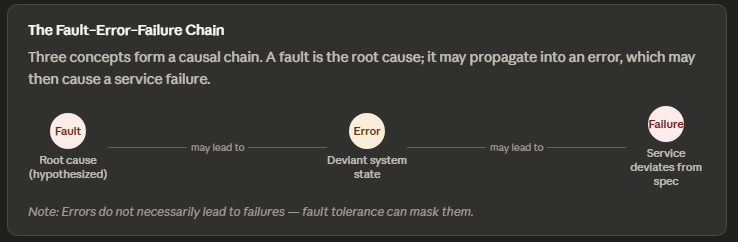
\includegraphics[width=0.8\linewidth]{figures/Lecture10/dependability.png}
    \label{fig:placeholder}
\end{figure}

% -------------------------------------------------------
\section*{Slide 3 — Attributes of Dependability}

Dependability is not a single metric but an umbrella concept with several 
attributes.
\begin{figure}[H]
    \centering
    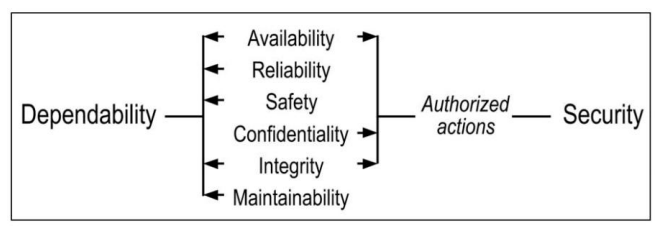
\includegraphics[width=0.7\linewidth]{figures/Lecture10/umbrella.png}
    \label{fig:placeholder}
\end{figure}

\begin{itemize}

    \item \textbf{Availability} asks whether the system is operational at any given moment. 
    A system with high availability is rarely down, and when it does fail it recovers 
    quickly. It tolerates failures as long as recovery is fast enough.

    \item \textbf{Reliability} is stricter — it asks whether the system has worked 
    continuously without interruption over some interval $[0, t]$. A system can have 
    high availability but low reliability if it fails and recovers frequently. Reliability 
    is the right metric for mission-critical systems where even a brief interruption 
    is unacceptable.

    \item \textbf{Safety} is concerned not with whether the system works, but with what 
    happens when it does not. A system can fail without being unsafe, but in domains 
    such as aviation or nuclear power, failures must not lead to catastrophic consequences 
    for users or the environment.

    \item \textbf{Integrity} asks whether the system has been altered in an unauthorized 
    or unintended way. A system can be available and reliable yet have compromised 
    integrity if its internal state or outputs cannot be trusted.

    \item \textbf{Maintainability} describes how easily a system can be repaired or 
    modified. It directly influences availability — fast repair keeps downtime short 
    even when failures are frequent.

    \item \textbf{Confidentiality} ensures information is only accessible to authorized 
    parties. When combined with enforcing authorized actions, it extends into the 
    broader notion of \textbf{security}.

\end{itemize}

\begin{keybox}
    Availability and reliability are the two attributes most commonly 
    quantified via Markov chains. The remaining attributes require 
    different modelling approaches.
    \begin{itemize}
        \item \textbf{Availability} asks whether the system is operational at any given moment
        \item \textbf{Reliability} is stricter — it asks whether the system has worked 
    continuously without interruption over some interval $[0, t]$. A system can have 
    high availability but low reliability if it fails and recovers frequently.
    \end{itemize}
    
\end{keybox}



% -------------------------------------------------------
\section*{Slide 4 — Binary System Model}
\begin{figure}[H]
    \centering
    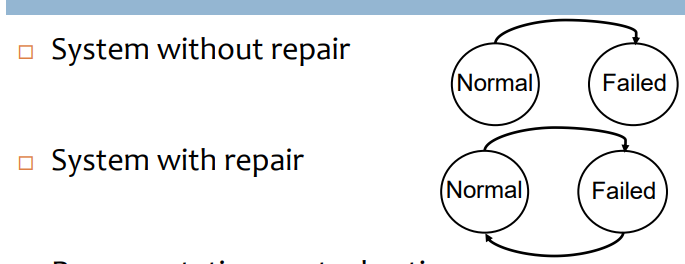
\includegraphics[width=0.7\linewidth]{figures/Lecture10/systemrepair.png}
    \label{fig:placeholder}
\end{figure}
A system is modelled as a binary stochastic process $S(t) \in \{0, 1\}$, 
where $S(t) = 1$ denotes the normal (operational) state and $S(t) = 0$ 
denotes the failed state. This gives precise probabilistic definitions:
\begin{align}
    A(t) &:= \Pr(S(t) = 1) \\[6pt]
    R(t) &:= \Pr\bigl(S(t') = 1 \text{ for all } t' \in [0,t]\bigr)
\end{align}
\begin{itemize}
    \item Availability $A(t)$ is a snapshot probability — it asks whether the system 
is up at time $t$, regardless of what happened before.
\item Reliability $R(t)$ 
is a path property — it asks whether the system has been continuously 
operational throughout the entire interval $[0, t]$.
\end{itemize}
\begin{warnbox}
    A single failure in $[0, t]$ sets $R(t) = 0$ for that sample path, So for reliability, once failure happens, we no longer care about repairs.

    However in an availability model, repairs matter.
    even if the system fully recovers afterward. However in an availability model, repairs matter, as you can go from an failed state to operational state.
    
    This is why availability 
    and reliability require different Markov models — the reliability model 
    uses an absorbing failed state, while the availability model allows 
    transitions back to the operational state.
\end{warnbox}

% -------------------------------------------------------
\section*{Slide 7 — Exponential Distributions}

The exponential distribution is the foundation of continuous-time Markov 
chain models. It is characterised by a single rate parameter $\lambda > 0$:

\begin{align}
    f(x)   &= \lambda e^{-\lambda x}, \quad x > 0 
             \tag{density} \\[4pt]
    F(x)   &= 1 - e^{-\lambda x} 
             \tag{CDF} \\[4pt]
    R(x)   &= e^{-\lambda x} 
             \tag{Reliability function} \\[4pt]
    \mathbb{E}[X] &= \frac{1}{\lambda}, \quad 
    \mathrm{Var}[X] = \frac{1}{\lambda^2}, \quad C^2 = 1
\end{align}

\begin{notebox}
    \textbf{Memoryless property:}
    \[
        \Pr(X > x + y \mid X > x) = e^{-\lambda y}
    \]
    The remaining lifetime of a component does not depend on how long it 
    has already been running. This is the property that makes the Markov 
    assumption valid.
\end{notebox}

Two further results are essential for multi-component modelling. If 
$X \sim \mathrm{Exp}(\lambda)$ and $Y \sim \mathrm{Exp}(\mu)$ are 
independent then:

\begin{align}
    \min(X, Y) &\sim \mathrm{Exp}(\lambda + \mu) \\[6pt]
    \Pr(X < Y) &= \frac{\lambda}{\lambda + \mu}
\end{align}

The first result gives the time to the first failure in a two-component 
system. The second determines which component fails first, and therefore 
which transition the Markov chain takes.
\todo{revised and look at}
% -------------------------------------------------------
\section*{Slide 8 — Discrete-Time Markov Chains}

A discrete-time Markov chain (DTMC) is defined on a finite or countably 
infinite state space $E = \{0, 1, 2, \ldots, K\}$. The transition 
probability $p_{jk}$ gives the probability of moving from state $j$ to 
state $k$ in one step. The \textbf{Markov property} states:

\[
    \Pr(X_i = k) = \sum_j \Pr(X_{i-1} = j) \cdot p_{jk}
\]

Writing $\pi_i$ as the row probability vector at step $i$ and $P$ as the 
transition matrix:

\begin{align}
    \pi_i &= \pi_{i-1} \cdot P \tag{transient} \\[6pt]
    \pi   &= \pi \cdot P, \quad \sum_i \pi_i = 1 \tag{steady state}
\end{align}

State holding times in a DTMC are geometrically distributed. The 
steady-state solution exists and is unique under three conditions:

\begin{notebox}
    \begin{itemize}
        \item \textbf{Irreducibility} — every state is reachable from 
        every other state (no absorbing states).
        \item \textbf{Non-periodicity} — states are not visited only at 
        multiples of some period $d > 1$.
        \item \textbf{Homogeneity} — transition probabilities are constant 
        over time.
    \end{itemize}
\end{notebox}
\todo{IDK what is happening here with pi and thing relook at}
\begin{warnbox}
    Reliability models intentionally violate irreducibility — the failed 
    state is absorbing, meaning once the system fails it cannot recover. 
    This is what distinguishes the reliability Markov model from the 
    availability model.
\end{warnbox}

% -------------------------------------------------------
\section*{Slide 9 — Continuous-Time Markov Chains}

A continuous-time Markov chain (CTMC) replaces transition probabilities 
with transition rates $\mu_{jk}$ (events per unit time). The time spent 
in state $j$ before leaving is exponentially distributed with rate 
$\Lambda(j) = \sum_{k \neq j} \mu_{jk}$, and the probability that the 
next transition goes to state $k$ is $\mu_{jk} / \Lambda(j)$.

The generator matrix $Q$ is an $n \times n$ matrix with off-diagonal 
entries $q_{ij} = \mu_{ij} > 0$ and diagonal entries chosen so that 
each row sums to zero:

\[
    q_{ii} = -\sum_{j \neq i} q_{ij}
\]

For a simple two-state system this gives:

\subsection*{The Generator Matrix $Q$}
\[
    Q = \begin{bmatrix} -q_{12} & q_{12} \\ q_{21} & -q_{21} \end{bmatrix}
\]
Think of $q_{12}$ as the rate at which the system moves from state 1 
to state 2, and $q_{21}$ as the rate back. If the mean time to failure 
is 10 time units then $q_{12} = 1/10 = 0.1$. If the mean time to repair 
is 1 time unit then $q_{21} = 1/1 = 1$. The diagonal entries are the 
negative row sum, which enforces that total probability is conserved --- 
the system must always be in some state.

\subsection*{The Transient Solution}
The transient state probabilities are governed by the 
Chapman-Kolmogorov equations:
\[
    \frac{d\pi_i(t)}{dt} = -\Lambda_i \cdot \pi_i(t) 
    + \sum_{j \neq i} \mu_{ji} \cdot \pi_j(t)
\]
In matrix form this is $\tfrac{dP(t)}{dt} = P(t) \cdot Q$, with solution:
\[
    P(t) = P(0) \cdot \mathrm{expm}(Qt)
\]
This gives the probability of being in each state at time $t$, given 
where the system started. $P(0)$ is the starting condition --- for 
example $P(0) = [1,\ 0]$ means the system starts operational with 
certainty. What you get out is a vector such as $[0.91,\ 0.09]$ at 
time $t = 5$, meaning there is a 91\% probability the system is 
operational at that moment.
\begin{warnbox}
    $P(t)$ gives you \textbf{availability} at time $t$, not reliability. 
    It answers the question: given where I started, what is the probability 
    the system is operational right now at time $t$? Reliability would 
    require a different $Q$ where the failed state is absorbing --- meaning 
    once the system fails it cannot recover, so any failure in $[0, t]$ 
    permanently counts against it.
\end{warnbox}

The matrix exponential $\mathrm{expm}(Qt)$ propagates the initial 
condition forward in time. This cannot be computed as a scalar 
exponential --- it requires the full matrix exponential 
(\texttt{expm} in MATLAB, \texttt{scipy.linalg.expm} in Python).

\subsection*{The Steady-State Solution}

\[
    \pi Q = 0, \qquad \pi \cdot \mathbf{1} = 1
\]

As $t \to \infty$, the transient solution $P(t)$ settles at a fixed 
distribution $\pi$. The equation $\pi Q = 0$ says the distribution 
is no longer evolving --- the flow of probability into each state 
exactly balances the flow out. The second equation enforces that 
probabilities sum to one. For the two-state example this gives the 
stationary availability directly:

\[
    \pi_1 = \frac{q_{21}}{q_{12} + q_{21}} = \frac{1}{1.1} \approx 0.909
\]

So in the long run the system is operational approximately 90.9\% 
of the time.

\begin{keybox}
    The transient solution $P(t)$ gives availability at a specific 
    time $t$ from a known starting state. The steady-state solution 
    $\pi$ gives the long-run average availability regardless of starting 
    state. For a full availability analysis you typically want both --- 
    the transient part shows how quickly the system converges, and $\pi_1$ 
    gives the asymptotic availability it converges to.
\end{keybox}
\todo[inline]{need to look at all here after}

\section*{Slide 11 — Markov Model: Single Component}

The simplest non-trivial model is a single component with two states: 
operational (state 1) and failed (state 2). The component has an 
exponentially distributed time to failure with mean $1/\lambda$ and 
an exponentially distributed time to repair with mean $1/\mu$. The 
generator matrix is:

\[
    Q = \begin{bmatrix} -\lambda & \lambda \\ \mu & -\mu \end{bmatrix}
\]

For the example on the slide, the mean time to failure is 10 and the 
mean time to repair is 1, giving $\lambda = 0.1$ and $\mu = 1$. The 
stationary availability is:

\[
    \pi_1 = \frac{\mu}{\lambda + \mu} = \frac{1}{1.1} \approx 0.909
\]

The transient availability $A(t) = P_1(t)$ is computed as:

\[
    P(t) = P(0) \cdot \mathrm{expm}(Qt)
\]

\begin{notebox}
    The initial condition $P(0)$ affects how $A(t)$ approaches the 
    steady state, but not the steady state itself:
    \begin{itemize}
        \item $P(0) = [1,\ 0]$: system starts operational, $A(t)$ 
        decreases toward $\pi_1$.
        \item $P(0) = [0,\ 1]$: system starts failed, $A(t)$ 
        increases toward $\pi_1$.
        \item $P(0) = [\pi_1,\ \pi_2]$: system starts at steady 
        state, $A(t)$ remains flat.
    \end{itemize}
    All three converge to the same stationary availability $\pi_1 
    \approx 0.909$.
\end{notebox}

\begin{warnbox}
    This model includes repair transitions, so $P(t)$ gives 
    \textbf{availability}, not reliability. For reliability the 
    repair transition $\mu$ must be removed, making state 2 absorbing. 
    $R(t)$ will then decay monotonically to zero, whereas $A(t)$ 
    converges to a non-zero steady state.
\end{warnbox}

% -------------------------------------------------------
\section*{Slide 12 — Multiple Components: Product State Space}

When a system has multiple components, the state space is formed as 
the product of the individual component state spaces. For two 
components $X$ and $Y$, each with states correct ($c$) and incorrect 
($i$), the four combined system states are:

\[
    (X_c, Y_c), \quad (X_i, Y_c), \quad (X_c, Y_i), \quad (X_i, Y_i)
\]

Whether a system state counts as operational depends on the system 
structure:

\begin{itemize}
    \item \textbf{Non-redundant (serial) system}: correct service 
    requires both components working. Only $(X_c, Y_c)$ is operational; 
    states $(X_i, Y_c)$, $(X_c, Y_i)$ and $(X_i, Y_i)$ are all failed.

    \item \textbf{Redundant (parallel) system}: correct service requires 
    at least one component working. States $(X_c, Y_c)$, $(X_i, Y_c)$ 
    and $(X_c, Y_i)$ are all operational; only $(X_i, Y_i)$ is failed.
\end{itemize}

\begin{notebox}
    The product state space construction is general --- for $n$ 
    components each with $k$ states, the combined state space has 
    $k^n$ states. The Markov chain is built on this combined space, 
    with transition rates inherited from the individual components.
\end{notebox}

% -------------------------------------------------------
\section*{Slide 13 — Redundant System: Reliability vs Availability}

For the redundant (parallel) two-component system, the reliability 
and availability models differ in which transitions are included.

In the \textbf{availability model}, repair transitions are present 
from all failed or degraded states back toward $(X_c, Y_c)$. The 
full generator matrix $Q$ is used and $A(t)$ converges to a 
non-zero steady state.

In the \textbf{reliability model}, repair transitions out of the 
fully failed state $(X_i, Y_i)$ are removed, making it absorbing. 
The reduced matrix $Q_{\mathrm{red}}$ retains only the operational 
and degraded states. $R(t)$ then decays monotonically to zero.

The two metrics are computed as:

\[
    R(t) = P_1(t,\, Q_{\mathrm{red}}) + P_2(t,\, Q_{\mathrm{red}}) 
    + P_3(t,\, Q_{\mathrm{red}})
\]

\[
    A(t) = P_1(t,\, Q) + P_2(t,\, Q) + P_3(t,\, Q)
\]

\begin{warnbox}
    The only structural difference between the two models is the 
    removal of repair transitions from the failed state. This makes 
    the failed state absorbing for reliability. Using the wrong model 
    --- for instance computing $R(t)$ with a $Q$ that includes repair 
    --- will give availability, not reliability, and the result will 
    never decay to zero.
\end{warnbox}

% -------------------------------------------------------
\section*{Slide 14 — Availability Computation}

For the redundant two-component system with failure rates $\lambda_X$, 
$\lambda_Y$ and repair rates $\mu_X$, $\mu_Y$, the full generator 
matrix is:

\[
Q = \begin{pmatrix}
-(\lambda_X + \lambda_Y) & \lambda_Y & \lambda_X & 0 \\
\mu_Y & -(\lambda_X + \mu_Y) & 0 & \lambda_X \\
\mu_X & 0 & -(\mu_X + \lambda_Y) & \lambda_Y \\
0 & \mu_X & \mu_Y & -(\mu_X + \mu_Y)
\end{pmatrix}
\]

The state ordering is $(X_c, Y_c)$, $(X_c, Y_i)$, $(X_i, Y_c)$, 
$(X_i, Y_i)$. Availability is the probability of being in any of 
the first three states:

\[
    A(t) = P_1(t) + P_2(t) + P_3(t) = P(t) \cdot \mathbf{1}_3^A
\]

where the summation vector $\mathbf{1}_3^A = (1,\ 1,\ 1,\ 0)^T$ 
selects the operational states. The transient solution is:

\[
    P(t) = P(0) \cdot \mathrm{expm}(Qt)
\]

\begin{notebox}
    Each row of $Q$ corresponds to a state. The off-diagonal entry 
    $q_{ij}$ is the rate of transitioning from state $i$ to state $j$. 
    For example, from the fully operational state $(X_c, Y_c)$ the 
    system can fail to $(X_c, Y_i)$ at rate $\lambda_Y$ or to 
    $(X_i, Y_c)$ at rate $\lambda_X$, giving a total departure rate 
    of $\lambda_X + \lambda_Y$ on the diagonal.
\end{notebox}

% -------------------------------------------------------
\section*{Slide 15 — Reliability Computation}

The reliability model uses the same state space but removes the 
repair transitions out of the fully failed state $(X_i, Y_i)$, 
making it absorbing. The reduced matrix $Q_{\mathrm{red}}$ is 
obtained by zeroing those repair rates. The solution is:

\[
    P(t) = P(0) \cdot \mathrm{expm}(Q_{\mathrm{red}}\, t)
\]

\[
    R(t) = P(t) \cdot \mathbf{1}_3^A, 
    \qquad \mathbf{1}_3^A = (1,\ 1,\ 1,\ 0)^T
\]

\begin{warnbox}
    Because $(X_i, Y_i)$ is now absorbing, probability flows into 
    it and never returns. $R(t)$ therefore decays monotonically to 
    zero --- the system will eventually fail permanently. This is 
    the correct behaviour for a reliability model with no repair.
\end{warnbox}

% -------------------------------------------------------
\section*{Slide 16 — Model Variants}

The base model can be modified to capture more realistic scenarios. 
The key question for each variant is: how does the modification 
change the transition rates in $Q$?

\textbf{Redundancy types.} In the base model both components are 
always active and can fail at any time. Two common alternatives are:

\begin{itemize}
    \item \textbf{Active stand-by}: only the active component can 
    fail. The stand-by component has zero failure rate until it is 
    activated. In the Markov chain, the failure rate of the stand-by 
    component is set to zero while it is in stand-by.

    \item \textbf{Activation on demand}: when the primary component 
    fails, the redundant one must be switched in. If activation is 
    instantaneous, the state transition happens immediately. If 
    activation takes an exponentially distributed time with mean $D$, 
    an intermediate activating state is added to the chain with 
    departure rate $1/D$.
\end{itemize}

\textbf{Correlated faults and repairs.} In the base model failure 
and repair rates are independent of the state of the other component. 
Correlation is modelled by making rates state-dependent:

\begin{itemize}
    \item If the failure rate of component $Y$ increases to 
    $\lambda_Y'$ whenever $X$ is failed, then the transition rate 
    from $(X_i, Y_c)$ to $(X_i, Y_i)$ becomes $\lambda_Y'$ instead 
    of $\lambda_Y$.

    \item If the repair rate degrades by 50\% when both components 
    are down, then the repair rates out of $(X_i, Y_i)$ become 
    $\mu_X / 2$ and $\mu_Y / 2$.
\end{itemize}

\begin{notebox}
    All of these variants are expressed purely as changes to the 
    entries of $Q$. The solution method --- $P(t) = P(0) \cdot 
    \mathrm{expm}(Qt)$ --- remains exactly the same regardless of 
    the variant.
\end{notebox}

% -------------------------------------------------------
\section*{Slide 17 — Modelling Multiple Fault Types}

A single component can be subject to several distinct fault types, 
each with its own failure rate and repair rate. For example:

\begin{itemize}
    \item Hardware fault: $\mathrm{mTTF}_1 = 100$, 
    $\mathrm{mTTR}_1 = 10$, so $\lambda_1 = 0.01$, $\mu_1 = 0.1$.
    \item Software fault: $\mathrm{mTTF}_2 = 10$, 
    $\mathrm{mTTR}_2 = 1$, so $\lambda_2 = 0.1$, $\mu_2 = 1$.
\end{itemize}

Each fault type gets its own failed state. The state space becomes:

\[
    \{\text{operational},\ \text{failed (HW)},\ \text{failed (SW)}\}
\]

The system transitions from operational to failed (HW) at rate 
$\lambda_1$ and to failed (SW) at rate $\lambda_2$. Repair brings 
it back to operational at rates $\mu_1$ and $\mu_2$ respectively.

\begin{notebox}
    For the \textbf{availability} model all repair transitions are 
    included and the chain is irreducible. For the \textbf{reliability} 
    model all failed states are made absorbing. In both cases 
    $Q$ is extended to accommodate the extra states but the solution 
    method is unchanged.
\end{notebox}

\begin{warnbox}
    If faults of one type can also occur while repair of another 
    type is ongoing, additional states are needed to represent 
    combinations such as (failed HW, failed SW simultaneously). 
    This increases the state space but is handled naturally by the 
    product state space construction from slide 12.
\end{warnbox}

% -------------------------------------------------------
\section*{Slide 18 — Non-Constant Failure Rates}

So far all failure and repair times have been assumed exponentially 
distributed, giving constant hazard rates. In practice many failure 
mechanisms follow a bath-tub shaped hazard rate:

\begin{itemize}
    \item \textbf{Early life}: high failure rate due to manufacturing 
    defects.
    \item \textbf{Useful life}: low, approximately constant failure rate.
    \item \textbf{Wear-out}: increasing failure rate due to ageing.
\end{itemize}

A non-constant hazard rate cannot be directly represented in a 
standard Markov chain, since the memoryless property requires 
constant rates. The solution is to approximate the distribution 
using multiple states, each representing a phase of the component's 
life.

% -------------------------------------------------------
\section*{Slide 19 — Non-Constant Failure Rates: Phase Approach}

The intuitive approach is to add states that track which phase of 
its lifetime the component is currently in:

\begin{itemize}
    \item \textbf{State 1}: early life phase, high failure rate 
    $\lambda_{\mathrm{high}}$.
    \item \textbf{State 2}: useful life phase, low failure rate 
    $\lambda_{\mathrm{low}}$.
    \item \textbf{State 3}: wear-out phase, high failure rate 
    $\lambda_{\mathrm{wear}}$.
\end{itemize}

The component transitions through these phases at rates that 
reflect the expected duration of each phase. Within each phase 
the failure rate is constant, so the Markov property holds locally. 
The overall effect approximates the non-constant hazard.

\begin{notebox}
    This is the idea behind \textbf{phase-type distributions} --- 
    any non-negative distribution can be approximated arbitrarily 
    closely by a mixture of exponential phases. The accuracy of 
    the approximation improves as more phases are added, at the 
    cost of a larger state space.
\end{notebox}

% -------------------------------------------------------
\section*{Slide 20 — Example: TMR Systems}

A Triple Modular Redundancy (TMR) system consists of three identical 
components $C_1$, $C_2$, $C_3$ and a voter $V$. The system operates 
correctly as long as at least two of the three components are 
functioning --- this is called a 2-out-of-3 system. Assuming a 
perfect voter and independent components each with reliability 
$R_c(t) = e^{-\lambda t}$, the system reliability is:

\[
    R(t) = 3\bigl(R_c(t)\bigr)^2 - 2\bigl(R_c(t)\bigr)^3
         = 3e^{-2\lambda t} - 2e^{-3\lambda t}
\]

The mean time to failure of a single component is $\mathrm{MTTF}_c 
= 1/\lambda$. For the TMR system:

\[
    \mathrm{MTTF}_{\mathrm{TMR}} = \frac{5}{6\lambda}
\]

\begin{warnbox}
    The TMR system has a \textbf{lower} MTTF than a single component. 
    This seems counterintuitive but follows directly from the formula 
    --- redundancy helps in the short term by keeping $R(t)$ higher 
    initially, but the system has more components that can fail, so 
    the expected time until the majority fails is shorter. TMR is 
    therefore beneficial only for short mission times where the 
    initial reliability improvement matters more than the long-run 
    MTTF.
\end{warnbox}

\begin{keybox}
    MTTF alone is not a sufficient characterisation of dependability. 
    Two systems can have the same MTTF but very different reliability 
    functions $R(t)$. Always examine the full $R(t)$ curve rather 
    than relying on a single summary statistic.
\end{keybox}


